\chapterpage{Methodology}
\mychapter{Methodology}
\label{chap:methodology}

\section{Research Design}

Generally, crowd counting methods are divided into two groups: detection based counting, that localises people (or heads) and counts the number of people (or heads) by the cardinality of the set of localisations and density based counting, in which a model estimates the density of people (or heads) on an image, and the count is recovered by spatial integration of the estimated density map~\cite{sindagi2018survey}. Detection based counting is generally accurate when people are sparse, easy to visually distinguish from each other, while it is less accurate when occluded by other persons or objects, which is just the regime in which density map regression works more accurately~\cite{Zhang2016}. This study proposes an adaptive hybrid design, which takes advantage of the fact that both families are not exclusively used to detect the frame, but rather one or the other is used, depending on the scene density evaluation, derived from preliminary detection evidence, and that the output of both families is passed to a fusion stage, not separately reported.

\begin{figure}[H]
	\centering
	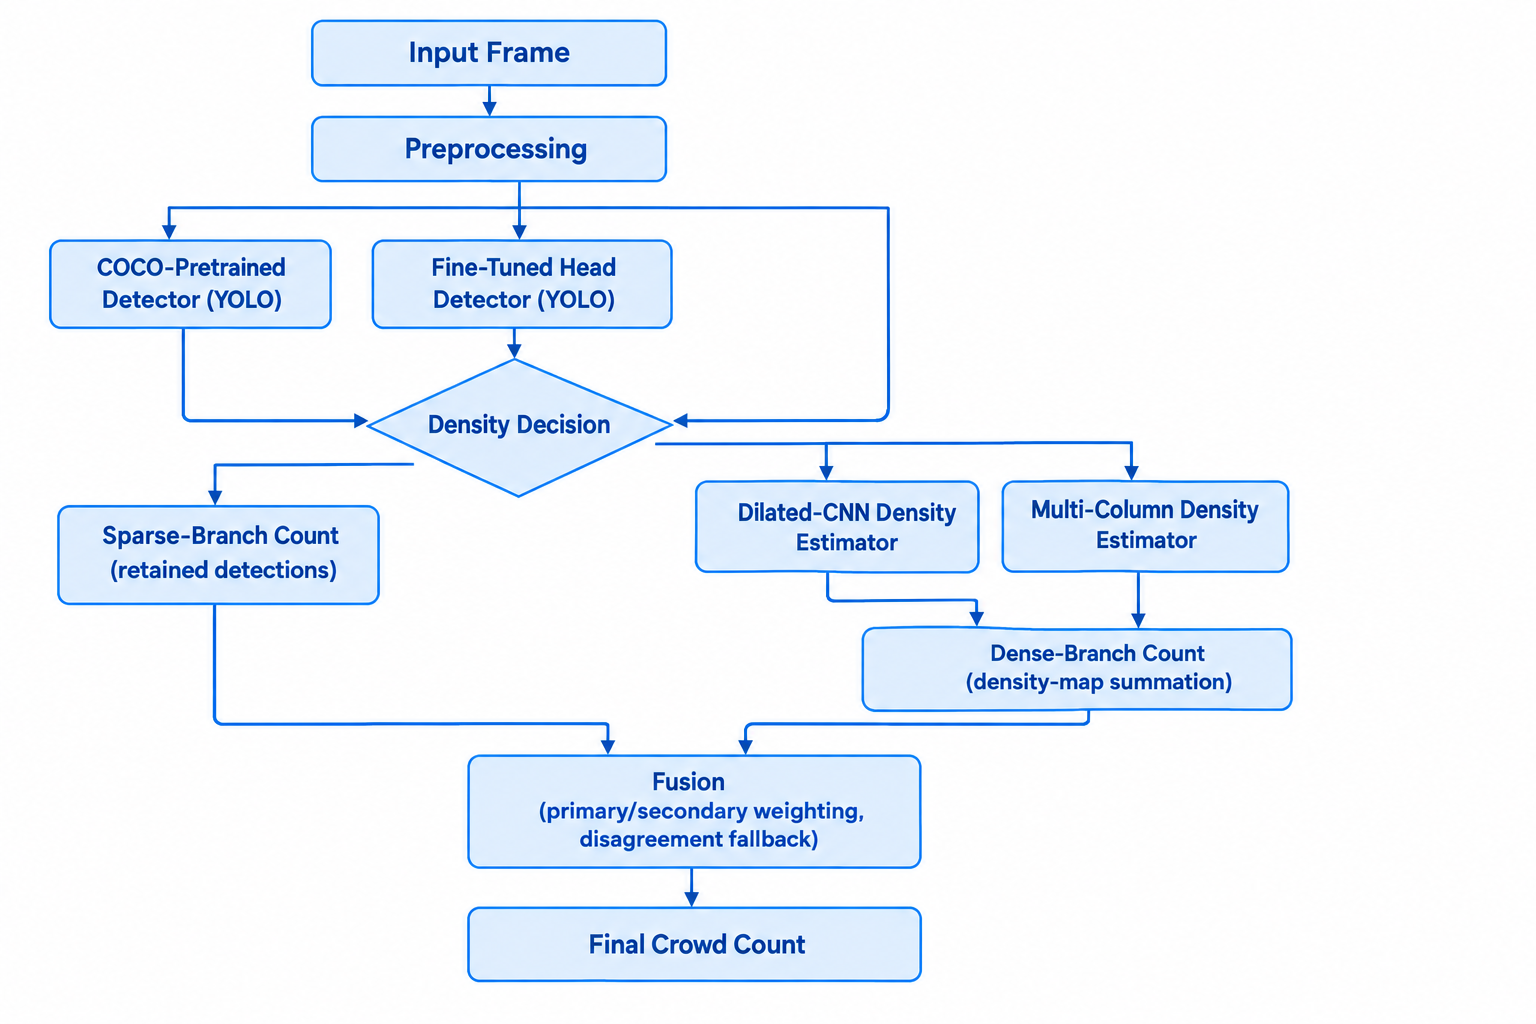
\includegraphics[width=0.92\textwidth]{./../images/pipeline_diagram.png}
	\caption{Architecture of the proposed adaptive hybrid crowd counting framework.}
	\label{fig:pipeline}
\end{figure}

The overall architecture is then five conceptual stages as illustrated in Figure~\ref{fig:pipeline}: (i) the input frame is passed to one or more candidate detector techniques; (ii) the outputs of the detector techniques are passed to a component that decides on whether the frame is sparse or dense based on the number of detections, detection density, and pairwise detection overlap; (iii) if the frame is dense, it is also passed to one of several candidate density estimation techniques, while if it is sparse, the detections are passed directly to a branch count component; (iv) both a sparse and a dense branch count are computed from the detections and passed to a (v) fusion component that reconciles the counts from the two branches into a single final crowd count, using one of several primary/secondary weighting schemes, with the secondary chosen whenever there is a strong disagreement between the two branches. 

\section{Research Approach}

This study is conducted in the above sequence of five stages and summarised for one frame in Table~\ref{tab:stages}. The two detector techniques and two density estimation techniques have different requirements for the preprocessed frames and require the input of a different set of frames, so each stage is examined separately in the corresponding subsection of Section~\ref{sec:proposed-algorithm}: frame preprocessing (technique specific), detection (Section~\ref{sec:sparse}), density decision (Section~\ref{sec:density-decision}), density estimation (Section~\ref{sec:dense}), and fusion (Section~\ref{sec:fusion}). The processing unit used throughout the rest of this chapter is a single frame and any detections that have been made for that frame; however, the way video frames are acquired and extracted from a video stream before this point is not examined here.

\begin{longtable}{|
		>{\raggedright\arraybackslash}p{0.19\textwidth}|
		>{\raggedright\arraybackslash}p{0.33\textwidth}|
		>{\raggedright\arraybackslash}p{0.38\textwidth}|}
	
	\caption{Stages of the research approach, from frame input to final count.}
	\label{tab:stages} \\
	
	\hline
	\textbf{Stage} & \textbf{Input} & \textbf{Output} \\
	\hline
	\endfirsthead
	
	\multicolumn{3}{c}%
	{{\tablename\ \thetable{} -- continued from previous page}} \\
	\hline
	\textbf{Stage} & \textbf{Input} & \textbf{Output} \\
	\hline
	\endhead
	
	\hline
	\multicolumn{3}{r}{{Continued on next page}} \\
	\endfoot
	
	\hline
	\endlastfoot
	
	Preprocessing
	&
	Raw frame
	&
	Model ready tensor (technique specific)
	\\
	\hline
	
	Detection
	&
	Preprocessed frame
	&
	Set of bounding box detections
	\\
	\hline
	
	Density decision
	&
	Detections and frame dimensions
	&
	Scene label (sparse/dense)
	\\
	\hline
	
	Sparse counting
	&
	Retained detections
	&
	Sparse branch count
	\\
	\hline
	
	Dense counting
	&
	Frame and, optionally, detections
	&
	Density map and dense branch count
	\\
	\hline
	
	Fusion
	&
	Sparse branch count, dense branch count, and scene label
	&
	Final crowd count
	\\
	\hline
	
\end{longtable}

\section{Data Analysis Techniques}
\label{sec:analysis-techniques}

As the sparse and dense branches produce structurally different outputs (discrete detections versus continuous density maps), and the classical, non-learned techniques (classical density estimation, density decision, fusion) are not trained against a loss function, each component of the framework is analysed with the metric family appropriate to its output.

\subsection{Image Pre-processing}

The preprocessor applies conditions on each frame before detection and density estimation using up to four optional, independently configurable stages, applied in sequence: resizing and scale normalization, non-local means denoising, Contrast Limited Adaptive Histogram Equalization (CLAHE) applied to the L-channel of the CIELAB colour space, and Gaussian smoothing. When a stage is disabled, its input passes through unchanged to the next stage.

\subsubsection{Resizing and Scale Normalization}

Before any denoising or contrast operation is applied, the raw frame $I_{raw}$ produced by input acquisition is resized to a standard working resolution:

\begin{equation}
	I_{in} = \operatorname{Resize}\left(I_{raw};\, \text{target}=w_{t},\, \text{interp}=\text{INTER\_AREA}\right), \qquad h_{t} = h_{raw} \cdot \frac{w_{t}}{w_{raw}}
	\label{eq:resize}
\end{equation}

where $w_t$ is the configured target width, $h_t$ the resulting target height, and the aspect ratio of the original frame $(w_{raw}, h_{raw})$ is preserved throughout. Area based interpolation is used because it is the theoretically appropriate choice for downscaling: unlike bilinear or nearest neighbour interpolation, which sample a fixed, small neighbourhood regardless of the scale change, area interpolation averages over the full block of source pixels each destination pixel covers, which reduces aliasing artefacts that would otherwise appear as spurious high frequency texture exactly the kind of artefact non-local means denoising would otherwise mistake for genuine, similarity matchable structure~\cite{gonzalez2018digital}.

\subsubsection{Non-Local Means Denoising}

Non-local means denoising~\cite{buades2005nonlocal} relies on the fact that in a crowd scene, similar texture and background regions occur many times throughout the image and the value of each pixel can be estimated by averaging with all the pixels in a search window where the surrounding patches are photometrically similar. denoised value of a pixel $p$ is

\begin{equation}
	I_{1}(p) = \frac{1}{C(p)} \sum_{q \in \Omega(p)} w(p,q)\, I_{in}(q)
	\label{eq:nlm-estimate}
\end{equation}
\begin{equation}
	w(p,q) = \exp\left(-\frac{\lVert N(p) - N(q) \rVert_2^2}{h^2}\right), \qquad C(p) = \sum_{q \in \Omega(p)} w(p,q)
	\label{eq:nlm-weight}
\end{equation}

The search window around $p$ ($\text{searchWindowSize}=21$), the local patches centred at $p$ and $q$ ($\text{templateWindowSize}=7$) used for similarity comparison, the filtering strength $h$ that controls the down weighting of dissimilar patches. In the case of colour images, denoising is done in the luminance chrominance decomposition with different strengths for luminance and colour channels, $h=3$ and $h_{color}=3$ respectively, respectively following the colour extension of the algorithm that suppress chroma noise without over smoothing brighteness edge. The spatial filter scheme, which depends only on the spatial distance between the two patches, does not preserve fine structure as well as the $w(p,q)$ scheme does because it does not consider similarity between the two patches.The fine structure (heads, edge of the occlusion boundary) is preserved better than a spatial filter scheme since the latter does not consider the similarity between the two patches. 

\subsubsection{Contrast Limited Adaptive Histogram Equalization}

\begin{equation}
	L' =
	\operatorname{CLAHE}\left(
	L;\,\text{clipLimit}=2.0,\,
	\text{tileGridSize}=8\times8
	\right)
	\label{eq:clahe}
\end{equation}

CLAHE partitions the $L$-channel into an $8\times8$ grid of contextual tiles, equalises the histogram within each tile, and clips histogram bins above a fixed limit (clipLimit $=2.0$) before redistributing the excess. This prevents noise over-amplification that plain histogram equalisation can introduce in near uniform regions~\cite{zuiderveld1994clahe}. Operating in the perceptually motivated CIELAB space isolates luminance from chrominance, so that contrast enhancement does not distort colour~\cite{lab_colorspace}. Applied to $I_1$ (or directly to $I_{in}$ if denoising is disabled), CLAHE improves local contrast in unevenly illuminated crowd scenes, such as shadowed platforms and backlit doorways. This enhancement can improve the recall of the downstream head/person detector, consistent with reported gains from CLAHE preprocessing in low contrast detection pipelines.

\subsubsection{Gaussian Smoothing}

\begin{equation}
	I_{out} =
	\operatorname{GaussianBlur}\left(
	I_{2};\,\text{kernel}=k_{blur},\,\sigma=0
	\right)
	\label{eq:gaussian-blur}
\end{equation}

A final, optional Gaussian smoothing pass with configurable kernel size $k_{blur}$ removes residual high-frequency artefacts introduced by CLAHE's per-tile equalisation before the frame is passed to the detection and density branches~\cite{gonzalez2018digital}. Setting $\sigma=0$ allows the Gaussian standard deviation to be determined automatically from the selected kernel size.

\subsection{ShanghaiTech Dataset Preparation}

The ShanghaiTech dataset is prepared for density based crowd estimation using a dedicated preprocessing pipeline. Each image and its corresponding head annotations are resized to a fixed resolution of $768\times768$, with the annotation coordinates scaled accordingly. Ground truth density maps are generated by placing unit impulses at the annotated head locations and applying an adaptive Gaussian kernel whose standard deviation depends on the number of annotated heads. The resulting density maps are normalized to preserve the ground truth crowd count and subsequently downsampled by a factor of four to match the spatial resolution of the density estimation network. A scaling factor of $16$ is applied after downsampling to compensate for the reduction in spatial resolution. Input images are converted to RGB format and normalized to the range $[0,1]$. The resulting image density map pairs provide the supervision required for training the multi column density estimator.

\section{Proposed Algorithm}
\label{sec:proposed-algorithm}

\subsection{Overall Proposed Framework}

The overall workflow of the proposed adaptive hybrid crowd counting framework is summarized in Algorithm~\ref{alg:overall}. It integrates density-based scene decision, sparse detection, dense estimation, and count fusion into a unified pipeline as shows in Figure~\ref{fig:pipeline}.

\begin{algorithm}[H]
	\caption{Adaptive Hybrid Crowd Counting}
	\label{alg:overall}
	\begin{algorithmic}[1]
		\Require Video $V$ or a single frame $f$
		\Ensure Final crowd count $C$
		\For{each frame $f_t$}
		\State Preprocess $f_t$ for the selected detector technique (Section~\ref{sec:sparse})
		\State $\mathcal{D} \gets$ detections produced by the selected detector technique
		\State $s \gets$ \Call{DensityDecision}{$\mathcal{D}$, dimensions of $f_t$} \Comment{Section~\ref{sec:density-decision}}
		\State $C_{\text{sparse}} \gets |\mathcal{D}|$ (after any confidence/class filtering, Section~\ref{sec:sparse})
		\State Preprocess $f_t$ for the selected density estimation technique
		\State $\hat D \gets$ density map from the selected density estimation technique (Section~\ref{sec:dense})
		\State $C_{\text{dense}} \gets \sum \hat D$ \Comment{Equation~\ref{eq:density-sum}}
		\State $C_t \gets$ \Call{Fuse}{$s$, $C_{\text{sparse}}$, $C_{\text{dense}}$} \Comment{Section~\ref{sec:fusion}}
		\EndFor
		\State $C \gets$ aggregation of $\{C_1,\dots,C_n\}$ across frames 
		\State \Return $C$
	\end{algorithmic}
\end{algorithm}

Note that both the sparse branch count and the dense branch count are computed for every frame, regardless of the scene label $s$ assigned by the density decision component, $s$ determines which of the two counts the fusion component treats as primary rather than determining which branch is computed at all (Section~\ref{sec:fusion}).

\subsection{Head Detection}
\label{sec:sparse-detection}

Two candidate techniques were implemented for the detection role, spanning a general purpose pretrained deep detector, a domain-fine-tuned deep detector. All two produce a common output representation, a set of bounding boxes, each optionally carrying a confidence score which downstream components (density decision, sparse counting, fusion) consume identically regardless of which technique produced it.

\subsection{Sparse Scene Crowd Counting}
\label{sec:sparse}

\subsubsection{Pretrained General Purpose Detector}

The first sparse branch technique employs the pretrained YOLOv8m object detector as a general-purpose person detector, as illustrated in Fig.~\ref{fig:sparse_yolov8_pretrained}. The model is loaded using the Ultralytics detection framework~\cite{yolov8_ultralytics} and is used without additional training or fine-tuning. During inference, the detector is configured with an input image size of $1024$ pixels, a confidence threshold of $0.25$, and the person class (class $0$). Therefore, only detections classified as persons with confidence scores satisfying the specified threshold are retained for counting.

\begin{figure}[htbp]
	\centering
	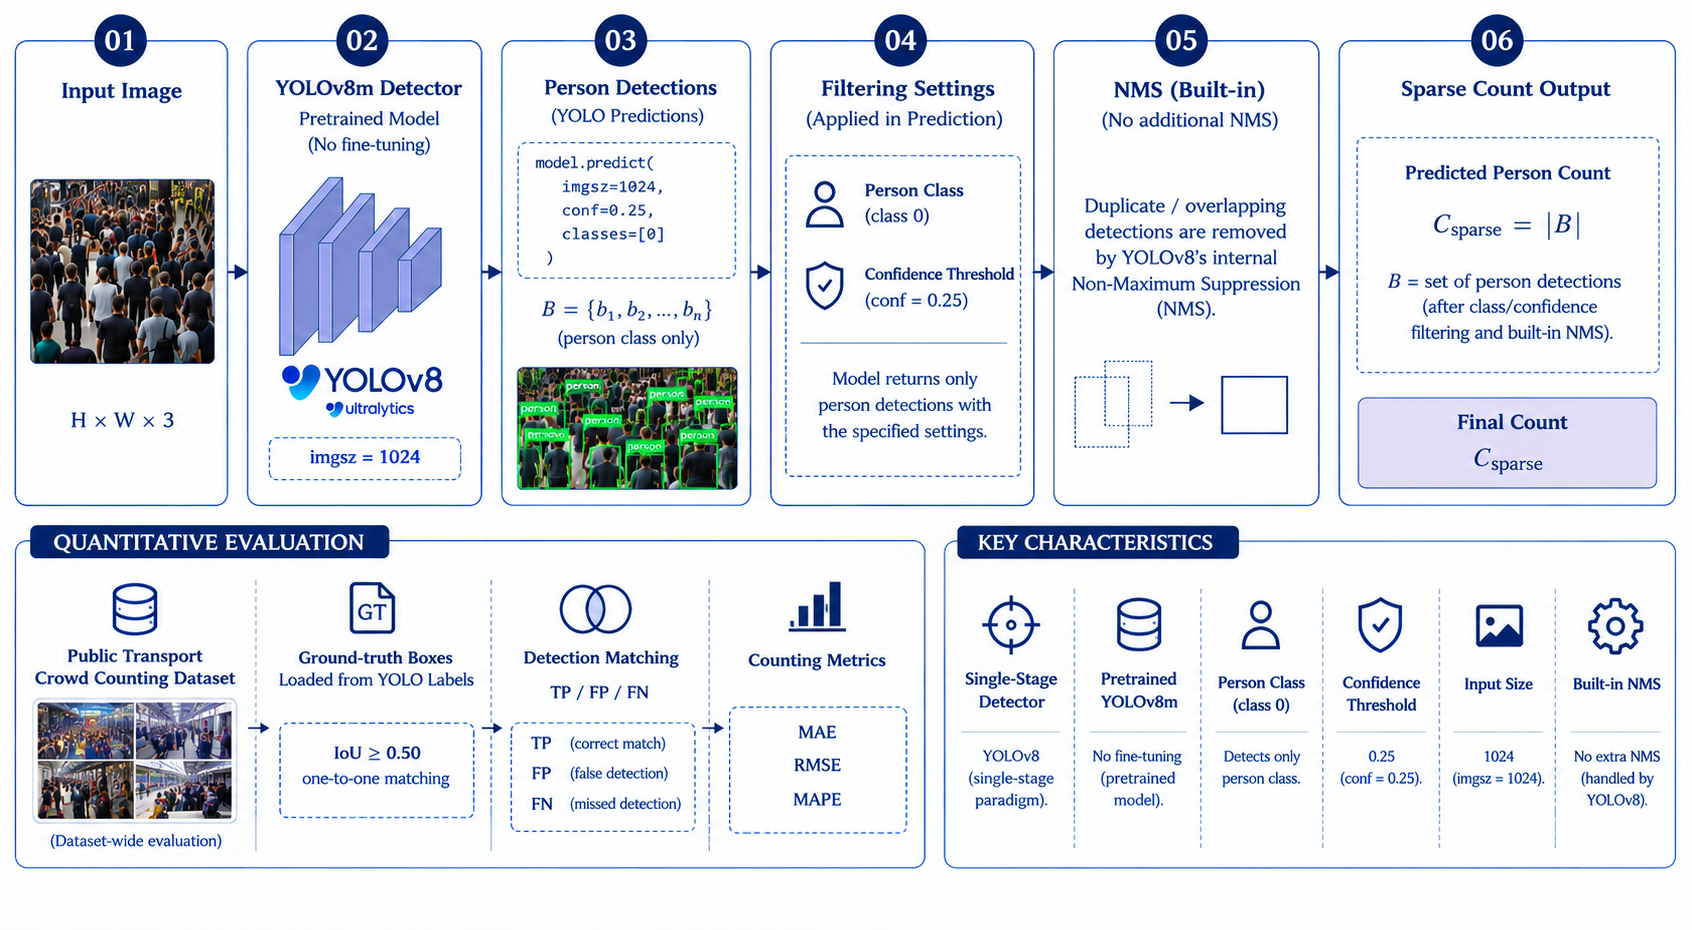
\includegraphics[width=\textwidth]{./../images/sparse/yolo/yolo_pretrained.png}
	\caption{Architecture of the pretrained YOLOv8 based sparse branch technique.}
	\label{fig:sparse_yolov8_pretrained}
\end{figure}

Let $B$ denote the set of bounding boxes returned by the pretrained YOLOv8m detector under the person class and confidence-threshold constraints. The sparse scene count is obtained directly from the number of retained detections:

\begin{equation}
C_{\text{sparse}} = |B|.
\end{equation}

The detector's built-in post-processing, including non-maximum suppression (NMS), is used to handle overlapping candidate detections, no additional NMS procedure is applied in the counting pipeline.

For quantitative evaluation, the predicted bounding boxes are compared with the ground truth bounding boxes provided with the public transport crowd counting dataset. A predicted box and a ground truth box are considered a match when their intersection-over-union (IoU) is at least $0.50$. A greedy one-to-one matching procedure is then used to determine true positives (TP), false positives (FP), and false negatives (FN). Based on these detections, precision, recall, and F1-score are calculated. In addition, counting performance is evaluated using the absolute counting error, mean absolute error (MAE), root mean squared error (RMSE), and mean absolute percentage error (MAPE).

\subsubsection{Fine-Tuned Head Detector}

The second sparse branch technique fine tunes the pretrained YOLOv8m detector for single class head detection using the SCUT-HEAD dataset~\cite{peng2018scuthead}, as illustrated in Fig.~\ref{fig:sparse_yolov8_head}. The detector is initialized from the pretrained YOLO weights and fine tuned for 50 epochs with a batch size of 8 and an input image size of 1{,}280 pixels. Early stopping is enabled with a patience of 10 epochs, while a fixed random seed of 42 and deterministic training are used to improve reproducibility. The dataset contains a single object class, namely \textit{head} (class 0).

\begin{figure}[htbp]
	\centering
	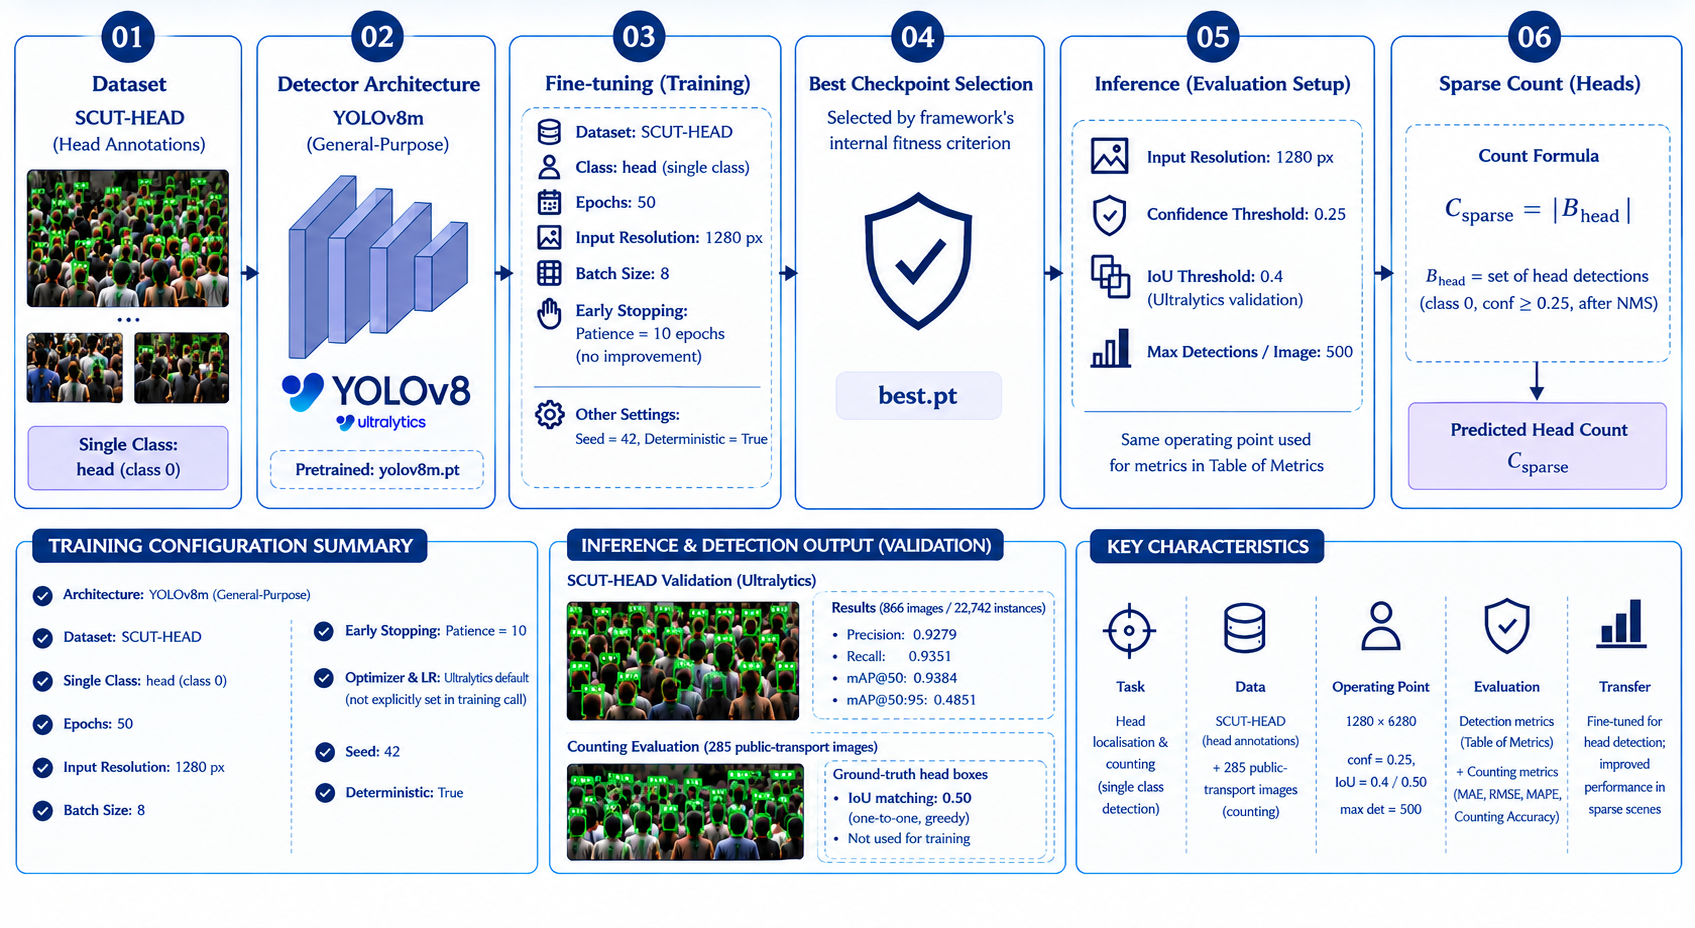
\includegraphics[width=\textwidth]{./../images/sparse/yolo/yolo_scut_head.png}
	\caption{Architecture of the fine-tuned YOLOv8 head detection technique.}
	\label{fig:sparse_yolov8_head}
\end{figure}

The Ultralytics validation procedure is performed at an input resolution of 1{,}280 pixels with a batch size of 8, a confidence threshold of 0.25, an IoU threshold of 0.4, and a maximum of 500 detections per image.

For sparse scene counting, the number of detected heads is obtained directly from the retained detection boxes. Let $B_{\text{head}}$ denote the set of head detections returned by the fine tuned detector after the specified class and confidence filtering. The sparse scene count is then calculated as

\begin{equation}
    C_{\text{sparse}} = |B_{\text{head}}|.
\end{equation}

No additional non-maximum suppression is applied outside the YOLO detection framework.

\subsubsection{Comparison of Sparse Branch Techniques}
\label{sec:sparse-comparison}

Table~\ref{tab:sparse-compare} summarizes the main characteristics of these two sparse branch techniques and provides a basis for selecting an appropriate detector within the proposed hybrid framework.

\begin{longtable}{|
    >{\raggedright\arraybackslash}p{0.22\textwidth}|
    >{\raggedright\arraybackslash}p{0.38\textwidth}|
    >{\raggedright\arraybackslash}p{0.32\textwidth}|}

\caption{Comparison of the two sparse branch (detection-based) techniques.}
\label{tab:sparse-compare}\\

\hline
\textbf{Aspect} &
\textbf{Pretrained Detector} &
\textbf{Fine-Tuned Detector} \\
\hline
\endfirsthead

\multicolumn{3}{c}%
{{\tablename\ \thetable{} -- continued from previous page}} \\
\hline
\textbf{Aspect} &
\textbf{Pretrained Detector} &
\textbf{Fine-Tuned Detector} \\
\hline
\endhead

\hline
\multicolumn{3}{r}{{Continued on next page}} \\
\endfoot

\hline
\endlastfoot

Underlying method
&
Deep, single stage regression detector~\cite{redmon2016yolo}
&
Same architecture, fine tuned
\\
\hline

Training performed
&
None (pretrained weights only)
&
Fine tuning, 50 epochs
\\
\hline

Target class
&
Person (general)
&
Head (domain specific)
\\
\hline

Confidence output
&
Graded score
&
Graded score
\\
\hline

Quantitative evaluation
&
None (qualitative only)
&
Detection metrics (Table~\ref{tab:metrics})
\\
\hline

\end{longtable}

\subsection{Density Decision}
\label{sec:density-decision}

The density decision component determines whether a frame is treated as sparse or dense, using only the detections produced by the upstream detector and the frame's spatial dimensions, it does not itself re-examine pixel content. Given a detection set $\mathcal{D} = \{d_1,\dots,d_n\}$ and a frame of height $h$ and width $w$, the component first normalises the frame area into units of 1{,}000 pixels$^2$,

\begin{equation}
	a = \frac{h \cdot w}{1000},
\end{equation}

and then applies a two stage rule. First, if the number of detections falls below a configured minimum threshold $\tau_{\min}$, the frame is classified as sparse immediately, without computing density or overlap (an efficiency short circuit for frames that are trivially uncrowded):

\begin{equation}
	n < \tau_{\min} \;\Rightarrow\; \text{scene} = \text{sparse}.
\end{equation}

Otherwise, two indicators are computed. The first is a detection \emph{density}, expressed as detections per 1{,}000 pixels$^2$ of frame area,

\begin{equation}
	\rho = \frac{n}{a} \qquad (a>0),
\end{equation}

and the second is a pairwise \emph{overlap ratio}, defined as the fraction of all unordered detection pairs whose bounding boxes have a nonzero Intersection-over-Union:

\begin{equation}
	\text{IoU}(d_i,d_j) = \frac{|\,\text{box}(d_i) \cap \text{box}(d_j)\,|}{|\,\text{box}(d_i) \cup \text{box}(d_j)\,|}, \qquad
	r = \frac{\bigl|\{(d_i,d_j) : \text{IoU}(d_i,d_j) > 0\}\bigr|}{\binom{n}{2}} \quad (n \ge 2),
\end{equation}

with $r = 0$ defined for $n<2$. The Intersection-over-Union quantity itself is the standard overlap measure used in object detection matching and non-maximum suppression~\cite{everingham2010voc}; here it is used not to suppress duplicate detections but to gauge how crowded (mutually occluding) the detected individuals are. The frame is classified as dense if either indicator exceeds its configured threshold,

\begin{equation}
	\rho \ge \tau_{\rho} \;\;\text{or}\;\; r \ge \tau_{r} \;\Rightarrow\; \text{scene} = \text{dense}, \qquad \text{otherwise scene} = \text{sparse},
\end{equation}

where $\tau_{\rho}$ (a density threshold, in detections per 1{,}000 pixels$^2$) and $\tau_{r}$ (an overlap ratio threshold in $[0,1]$) are configured constants. This rule means a frame can be classified dense either because it contains many detections relative to its area, or because a large fraction of its detections mutually overlap, even if the absolute detection count is moderate, capturing two distinct visual symptoms of crowding (numerosity and occlusion) with a single decision. 

\subsection{Dense Scene Crowd Counting}
\label{sec:dense}

\subsubsection{Ground truth density maps}

For each training image, a ground truth density map is constructed by placing a unit impulse at each annotated head location after rescaling the annotation coordinates to the network's fixed input resolution of $768{\times}768$. The resulting point map is smoothed using a Gaussian filter with a standard deviation

\begin{equation}
	\sigma =
	\begin{cases}
		0.5\,\sigma_{\text{base}}, & N > 100 \\
		\sigma_{\text{base}}, & N \le 100
	\end{cases}
	\qquad \sigma_{\text{base}} = 5,
\end{equation}

where $N$ is the number of annotated heads in the image. Thus, images containing more than 100 annotated heads use $\sigma=2.5$, whereas images with 100 or fewer heads use $\sigma=5$. After Gaussian smoothing, the density map is renormalised so that its total mass equals the ground truth head count $N$. The density map is subsequently downsampled by a factor of four to match the spatial resolution of the network output. Because the downsampling factor is four in each spatial dimension, the density values are multiplied by $4^2=16$ to compensate for the spatial reduction.

\subsubsection{Multi Column Density Estimator}
\label{sec:fourcolumn-density}

\begin{figure}[htbp]
	\centering
	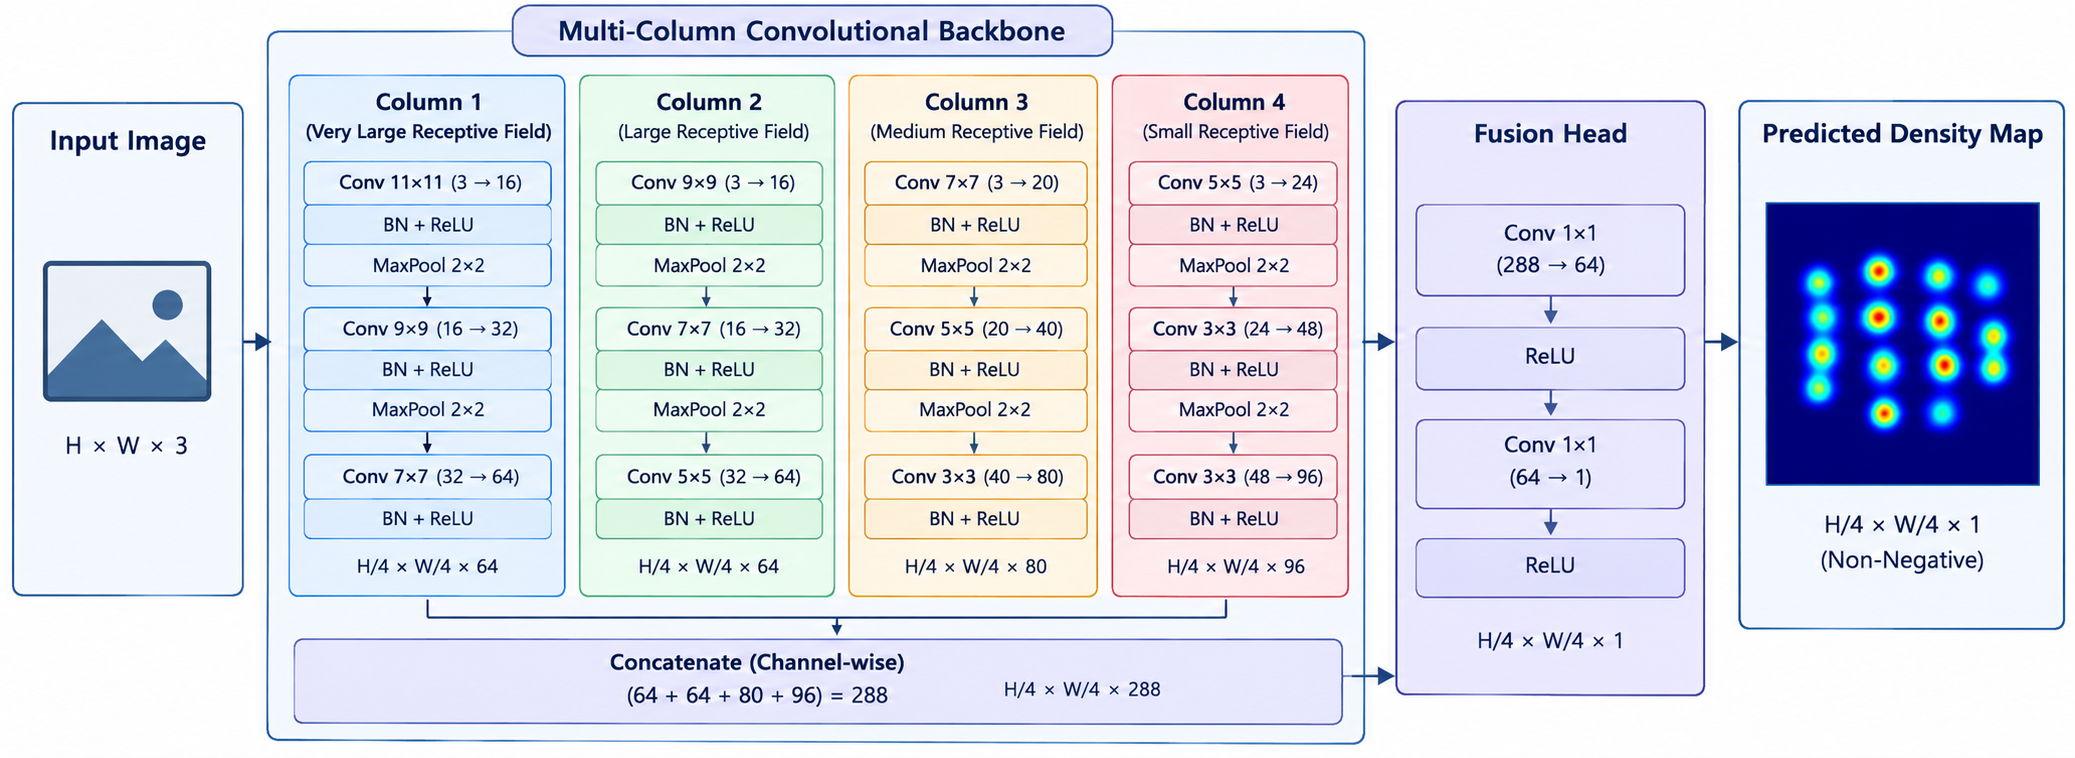
\includegraphics[width=\textwidth]{./../images/dense/mcnn/architecture.png}
	\caption{Architecture of Multi Column Density Estimator}
	\label{fig:multi_column_architecture}
\end{figure}

The first learned density estimation method is along the lines of the multi column convolutional architecture introduced by ~\cite{Zhu2020} (see Figure~\ref{fig:multi_column_architecture}) where multiple stacked parallel convolutional columns are trained on the same image, where each column uses a different kernel size to learn features for a different range of head sizes due to perspective and scale variations. Four parallel columns are used, with progressively smaller kernel sizes across the columns: the first column uses kernel sizes $11/9/7$, the second uses $9/7/5$, the third uses $7/5/3$, and the fourth uses $5/3/3$. The channel widths increase across the columns, with the four branches producing 64, 64, 80, and 96 output channels, respectively. Each convolution is followed by batch normalisation and ReLU activation, while two $2{\times}2$ max-pooling operations in each column reduce the spatial resolution by a factor of four. Thus, for the fixed input resolution of $768{\times}768$, all four branches produce feature maps of spatial size $192{\times}192$. The four feature maps are concatenated channel-wise, producing 304 channels, and are then passed through a fusion head consisting of a $1{\times}1$ convolution that reduces the channels from 304 to 64, followed by ReLU, and a second $1{\times}1$ convolution that produces a single channel output. A final ReLU ensures non-negative density values, yielding the predicted density map $\hat D$.

\subsubsection{Dilated Convolution Density Estimator}
\label{sec:csrnet-density}

\begin{figure}[htbp]
	\centering
	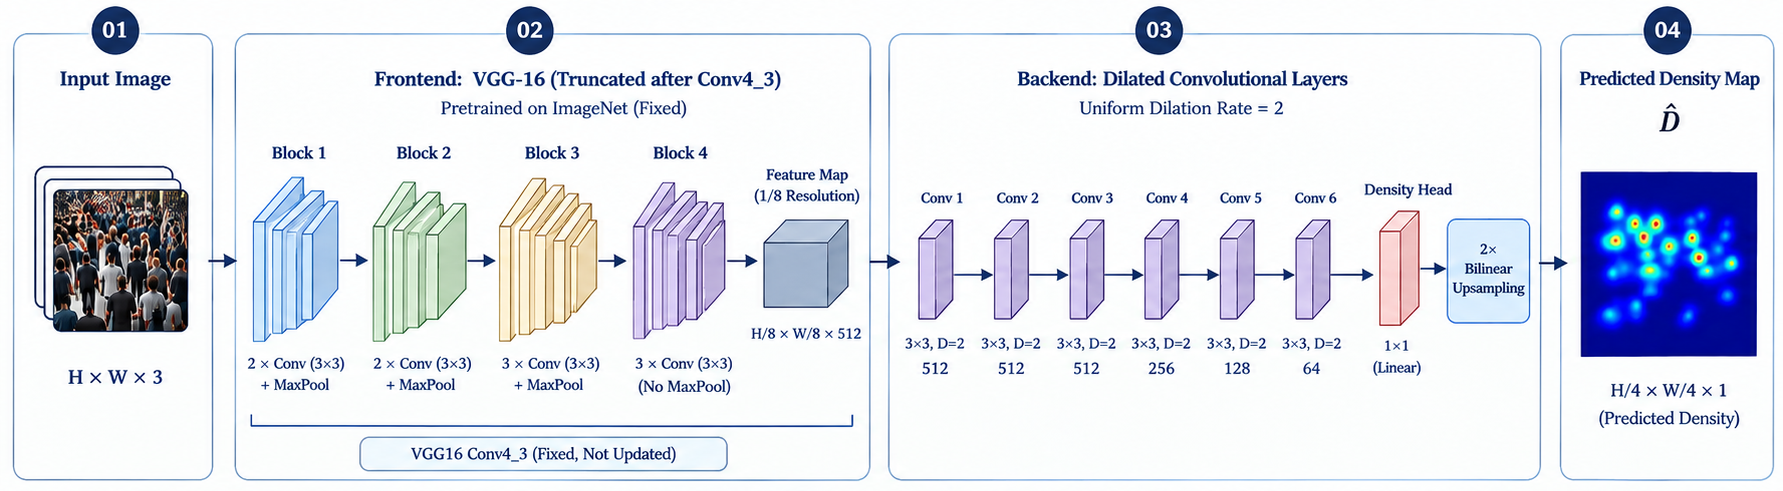
\includegraphics[width=\textwidth]{./../images/dense/csrnet/architecture.png}
	\caption{Architecture of Dilated Convolution Density Estimator.}
	\label{fig:csrnet_architecture}
\end{figure}

The second learned density estimation technique follows a two-part frontend and backend design based on the CSRNet architecture for congested scene density regression~\cite{li2018csrnet}, as illustrated in Figure~\ref{fig:csrnet_architecture}. The frontend is based on a VGG16 convolutional network pretrained on ImageNet~\cite{simonyan2015vgg}. The VGG16 feature extractor is truncated after the \texttt{conv4\_3} layer, corresponding to the fourth convolutional block. The frontend reduces the spatial resolution of the input from $768 \times 768$ to $96 \times 96$, while the pretrained frontend parameters are frozen during training and are therefore not updated.

The backend consists of six $3{\times}3$ convolutional layers with a uniform dilation rate of 2 and output channel sizes of 512, 512, 512, 256, 128, and 64. The dilated convolutions enlarge the receptive field while maintaining the $96{\times}96$ spatial resolution. A final $1{\times}1$ convolution reduces the 64 channel feature representation to a single channel density map. The predicted density map is subsequently upsampled by a factor of 2 using bilinear interpolation, producing a final spatial resolution of $192{\times}192$.

\subsubsection{Training}

The network is trained from randomly initialised weights using the Adam optimiser with an initial learning rate of $1\times10^{-4}$ and a batch size of 8. A StepLR learning rate scheduler is used with a step size of 10 epochs and a multiplicative factor of 0.1. Training is configured for a maximum of 100 epochs with early stopping using a patience of 30 epochs, and the checkpoint with the lowest validation loss is retained as the best model. The training objective is a weighted combination of pixel wise density map error and count level error,

\begin{equation}
	\mathcal{L} = 0.9 \, \mathcal{L}_{\text{MSE}}(\hat D, D) + 0.1 \, \bigl|{\textstyle\sum}\hat D - N_{gt}\bigr|,
\end{equation}

where the count level loss is computed using the absolute difference between the predicted and ground truth counts. For an individual sample, the predicted count is obtained by summing all values in the predicted density map,

\begin{equation}
	\hat C=\sum_{x,y}\hat D(x,y),
\end{equation}

and the count loss is

\begin{equation}
	\mathcal{L}_{\text{count}}=|\hat C-N_{\text{gt}}|.
\end{equation}

For a training batch, the implemented $\mathrm{L1Loss}$ computes the mean absolute count error across the samples. Input images are converted to RGB, resized to $768{\times}768$, and normalised to the range $[0,1]$ by division by 255, without additional channel-wise normalisation. No image augmentation is applied in the training configuration.

\subsubsection{Comparison of Dense Branch Techniques}
\label{sec:dense-comparison}

Table~\ref{tab:dense-compare} compares the two dense branch techniques in terms of their architectural design, density estimation capability, computational complexity, and overall suitability for handling variations in crowd density.

\begin{longtable}{|
	>{\raggedright\arraybackslash}p{0.22\textwidth}|
	>{\raggedright\arraybackslash}p{0.36\textwidth}|
	>{\raggedright\arraybackslash}p{0.34\textwidth}|}

\caption{Comparison of the two dense branch (density estimation) techniques.}
\label{tab:dense-compare}\\

\hline
\textbf{Aspect} &
\textbf{Multi-column Estimator} &
\textbf{Dilated CNN Estimator} \\
\hline
\endfirsthead

\multicolumn{3}{c}%
{{\tablename\ \thetable{} -- continued from previous page}} \\
\hline
\textbf{Aspect} &
\textbf{Multi-column Estimator} &
\textbf{Dilated CNN Estimator} \\
\hline
\endhead

\hline
\multicolumn{3}{r}{{Continued on next page}} \\
\endfoot

\hline
\endlastfoot

Underlying method
&
Multi-column CNN~\cite{Zhu2020}
&
VGG frontend + dilated backend~\cite{li2018csrnet, simonyan2015vgg}
\\
\hline

Learned parameters
&
Yes (trained from scratch)
&
Yes (frontend pretrained and frozen; backend trained)
\\
\hline

Depends on a detector
&
No
&
No
\\
\hline

ground truth smoothing $\sigma$
&
Adaptive: 5 or 2.5 by crowd size
&
Fixed: 4
\\
\hline

Training loss
&
$0.9\,\mathcal{L}_{\mathrm{MSE}} + 0.1\,\left|\sum \hat{D} - N_{\mathrm{gt}}\right|$
&
$\mathcal{L}_{\mathrm{MSE}}$ only
\\
\hline

\end{longtable}

\subsection{Fusion and Final Crowd Count}
\label{sec:fusion}

The fusion component reconciles the sparse branch count $C_{\text{sparse}}$ and the dense branch count $C_{\text{dense}}$, both of which are computed for every frame regardless of the scene label $s$ assigned by the density decision component, into a single final count for that frame. The scene label determines which of the two branch counts is treated as primary and which as secondary:

\begin{equation}
	(P,S) =
	\begin{cases}
		(C_{\text{sparse}}, C_{\text{dense}}), & s = \text{sparse} \\
		(C_{\text{dense}}, C_{\text{sparse}}), & s = \text{dense}
	\end{cases}
\end{equation}

with corresponding weights $(w_P,w_S)$ drawn analogously from a pair of configured branch weights (a sparse weight and a dense weight). If the primary count is non positive, the fusion component falls back to whichever of the two counts is larger, avoiding a zero final count when the primary branch reports nothing but the secondary branch has positive signal:

\begin{equation}
	P \le 0 \;\Rightarrow\; C = \max(P,S).
\end{equation}

Otherwise, a relative disagreement between the two branches is computed,

\begin{equation}
	\Delta = \frac{|P-S|}{P},
\end{equation}

and if this disagreement exceeds a configured threshold $\tau_{\Delta}$, the branches are judged too discordant to blend meaningfully, and the fusion component reports the primary count alone, trusting the branch that the density decision component identified as authoritative for that frame:

\begin{equation}
	\Delta > \tau_{\Delta} \;\Rightarrow\; C = P.
\end{equation}
Otherwise, the final count is a weighted average of the two branch counts,
\begin{equation}
	\Delta \le \tau_{\Delta} \;\Rightarrow\; C = \frac{P\,w_P + S\,w_S}{w_P + w_S}.
\end{equation}

The reason for this design is that the fusion component only blends the two branches where they are in reasonable agreement, and does not blend two potentially incommensurate density estimates, but rather just defers to the branch the density decision chose to take the lead.

\subsection{Evaluation Metrics}
\label{subsec:evaluation-metrics}

The evaluation strategy uses metrics appropriate to each component of the proposed crowd counting framework. The sparse detection branch is assessed using precision, recall, mAP@50, and mAP@50:95, while the learned density estimators are evaluated using pixel wise MSE, MAE, and count level MAE. The classical density estimator and deterministic density fusion components do not require training based metrics; instead, their outputs are assessed through diagnostic counts and fixed decision rules. Table~\ref{tab:metrics} summarizes the evaluation approach for each component.

\begin{longtable}{|
		>{\raggedright\arraybackslash}p{0.24\textwidth}|
		>{\raggedright\arraybackslash}p{0.33\textwidth}|
		>{\raggedright\arraybackslash}p{0.33\textwidth}|}
	
	\caption{Evaluation approach by component.}
	\label{tab:metrics}\\
	
	\hline
	\textbf{Component} &
	\textbf{Quantitative Evaluation Implemented} &
	\textbf{Notes} \\
	\hline
	\endfirsthead
	
	\multicolumn{3}{c}%
	{{\tablename\ \thetable{} -- continued from previous page}} \\
	\hline
	\textbf{Component} &
	\textbf{Quantitative Evaluation Implemented} &
	\textbf{Notes} \\
	\hline
	\endhead
	
	\hline
	\multicolumn{3}{r}{{Continued on next page}} \\
	\endfoot
	
	\hline
	\endlastfoot
	
	Pretrained sparse detector
	&
	Precision, recall, mAP@50, mAP@50:95
	&
	Single image, qualitative demonstration only
	\\
	\hline
	
	Fine tuned sparse detector
	&
	Precision, recall, mAP@50, mAP@50:95
	&
	Standard detection metrics at a fixed confidence/IoU operating point
	\\
	\hline
		
	Dilated CNN density estimator
	&
	Pixel wise MSE (training loss), pixel wise MAE, and custom count level MAE
	&
	Count level MAE compares summed predicted and ground truth density maps per batch
	\\
	\hline
	
	Multi column density estimator
	&
	Combined pixel wise MSE $+$ count level MAE (training loss); count level MAE tracked separately
	&
	Weighted combination, with weights fixed in the implementation
	\\
	\hline
	
\end{longtable}

\subsubsection{Count Based Evaluation Metrics}

For the sparse and dense branch evaluation, the following whole image count metrics are used, with $\hat c_i$ the predicted count and $c_i$ the ground truth count for image $i$ of $M$ evaluated images:

\begin{equation}
	\text{MAE} = \frac{1}{M}\sum_{i=1}^{M} \left| \hat{c}_i - c_i \right|, \qquad
	\text{RMSE} = \sqrt{ \frac{1}{M}\sum_{i=1}^{M} \left( \hat{c}_i - c_i \right)^2 }
\end{equation}

\begin{equation}
	\text{MAPE} = \frac{1}{M}\sum_{i=1}^{M} \frac{\left| \hat{c}_i - c_i \right|}{c_i} \times 100\%, \qquad
	\text{Bias} = \frac{1}{M}\sum_{i=1}^{M} \left( \hat{c}_i - c_i \right)
\end{equation}

RMSE penalises large individual errors more heavily than MAE, so a wide MAE/RMSE gap indicates that error is concentrated in a minority of images rather than spread evenly. Bias indicates systematic direction: a negative value indicates the model under counts on average. All four metrics are lower-is-better; bias is exceptional in that its \emph{sign}, not only its magnitude, is informative.

\subsubsection{Detection Metrics (Fine Tuned Sparse Detector)}

Detection quality is evaluated using precision ($P$), recall ($R$), and mean Average Precision (mAP), computed from matched predicted and ground truth bounding boxes. The evaluation follows the object detection protocol formalised for the PASCAL Visual Object Classes challenge~\cite{everingham2010voc}. In this study, detection performance is evaluated using a confidence threshold of 0.25, an Intersection-over-Union (IoU) threshold of 0.4, and a maximum of 500 detections per image. These settings are applied to the best checkpoint obtained during fine tuning.

\textbf{Precision} measures the proportion of predicted head boxes that correspond to ground truth heads. It is defined as:

\begin{equation}
	P = \frac{TP}{TP + FP},
\end{equation}

where $TP$ (true positives) represents the number of predicted boxes that sufficiently overlap with a ground truth head, while $FP$ (false positives) represents predictions that do not correspond to a ground truth head. Higher precision indicates fewer spurious detections.

\textbf{Recall} measures the proportion of ground truth heads that are successfully detected. It is defined as:

\begin{equation}
	R = \frac{TP}{TP + FN},
\end{equation}

where $FN$ (false negatives) represents the number of ground truth heads for which no corresponding prediction is obtained. Higher recall indicates fewer missed heads.

\textbf{Mean Average Precision (mAP)} provides a comprehensive measure of detection performance by summarising precision across the range of confidence thresholds. For \textbf{mAP@50}, Average Precision (AP) is calculated at a single IoU threshold of 0.50. The IoU between a predicted bounding box $A$ and a ground truth bounding box $B$ is defined as:

\begin{equation}
	\text{IoU}(A,B) = \frac{|A \cap B|}{|A \cup B|},
\end{equation}

while Average Precision is expressed as:

\begin{equation}
	\text{AP} = \int_0^1 p(r),dr,
\end{equation}

where $p(r)$ represents precision as a function of recall $r$.

The \textbf{mAP@50} metric therefore measures Average Precision at an IoU threshold of 0.50. In contrast, \textbf{mAP@50:95} averages AP across ten IoU thresholds from 0.50 to 0.95 in steps of 0.05. Consequently, mAP@50:95 provides a stricter and more localisation sensitive assessment of detection performance than mAP@50. For all three metrics, higher values indicate better detection performance.

\subsubsection{Density Estimation Training Metrics (Learned Dense Branch Estimators)}

Both learned density estimation techniques are trained with a pixel wise error term between the predicted density map $\hat D$ and the ground truth density map $D$,

\begin{equation}
	\mathcal{L}_{\text{MSE}} = \frac{1}{N_p}\sum_{i=1}^{N_p}\left(\hat D_i - D_i\right)^2,
\end{equation}

where $N_p$ is the number of cells in the (downsampled) density map. In addition, both techniques track a count level error metric that compares the summed predicted and ground truth density maps rather than their per-pixel values, expressed for a batch of size $B$ as

\begin{equation}
	\text{count\_MAE} = \frac{1}{B}\sum_{b=1}^{B}\left|\sum_{i} D_{b,i} - \sum_{i} \hat D_{b,i}\right|.
\end{equation}

This count level metric is used because pixel wise error on a density map is difficult to interpret directly in terms of people counted; expressing error in the same units as the final deliverable (a count) makes model comparison more directly meaningful. One of the two learned estimators uses only the pixel wise MSE as its training loss (with pixel wise MAE and count level MAE tracked as auxiliary metrics), while the other combines the pixel wise MSE and the count level error directly into its training loss (Section~\ref{sec:dense}).

\subsubsection{Count Derivation from a Density Map}

For any density estimation technique, learned or classical, the predicted crowd count $\hat C$ for a frame is obtained by spatial summation of the predicted density map,

\begin{equation}
	\hat C = \sum_{i=1}^{N_p} \hat D_i .
	\label{eq:density-sum}
\end{equation}

This relationship holds for the two learned estimators (where it is used directly in computing the count level MAE metric above) and, in a closed form variant, for the classical estimator.